\section{Image Stuff}

% Demonstrate basic image - https://www.overleaf.com/learn/latex/Inserting_Images
Including images in your document is easy \emoji{coolAndGood.png}
% Reference figure
To reference a figure we can label it, like it is done in figure \ref{fig:cake}.
% Demonstrate more complete image inclusion - https://www.overleaf.com/learn/latex/Positioning_images_and_tables
% Use [H] from `\usepackage{float}` to keep figure exactly here
\begin{figure}[H]
	\centering
	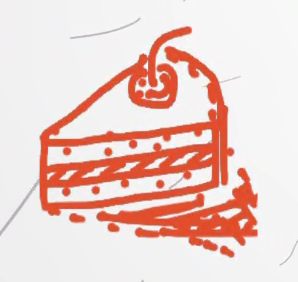
\includegraphics[width=0.3\textwidth]{cake}
	\captionsetup{justification=centering}
	\caption{
		This is not a cake \cite{magritte}, \\
		but a mere simulacrum \cite{beaudrillard}. \\
		$\therefore$ The `cake', as it were, is a lie \cite{rattman}.
	}
	\label{fig:cake}
\end{figure}

When the sunlight strikes raindrops in the air, they act as a prism and form a rainbow. The rainbow is a division of white light into many beautiful colors. These take the shape of a long round arch, with its path high above, and its two ends apparently beyond the horizon. There is , according to legend, a boiling pot of gold at one end. People look, but no one ever finds it. When a man looks for something beyond his reach, his friends say he is looking for the pot of gold at the end of the rainbow.
% Demonstrate wrapping figure
\begin{wrapfigure}{r}{6cm}
	\centering
	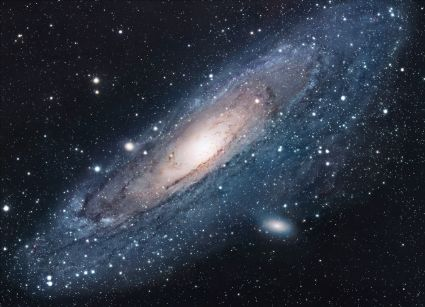
\includegraphics[width=0.8\linewidth]{universe}
	\caption*{\small Claustrophobia vs. Agoraphobia.}
\end{wrapfigure}
Throughout the centuries people have explained the rainbow in various ways. Some have accepted it as a miracle without physical explanation. To the Hebrews it was a token that there would be no more universal floods. The Greeks used to imagine that it was a sign from the gods to foretell war or heavy rain. The Norsemen considered the rainbow as a bridge over which the gods passed from earth to their home in the sky. Others have tried to explain the phenomenon physically. Aristotle thought that the rainbow was caused by reflection of the sun’s rays by the rain. Since then physicists have found that it is not reflection, but refraction by the raindrops which causes the rainbows. Many complicated ideas about the rainbow have been formed. The difference in the rainbow depends considerably upon the size of the drops, and the width of the colored band increases as the size of the drops increases. The actual primary rainbow observed is said to be the effect of super-imposition of a number of bows. If the red of the second bow falls upon the green of the first, the result is to give a bow with an abnormally wide yellow band, since red and green light when mixed form yellow. This is a very common type of bow, one showing mainly red and yellow, with little or no green or blue. % http://www.voxforge.org/home/submitspeech/windows/step-1/dialect/rainbow

% Demonstrate multiple vector figures
\begin{figure}[H]
	\centering
	\begin{subfigure}{0.45\textwidth}
		\centering
		
\includegraphics[width=0.7\textwidth]{potted_plant} 
		\caption{It's a potted plant!}
		\label{fig:potted}
	\end{subfigure}
	\begin{subfigure}{0.45\textwidth}
		\centering
		
\includegraphics[width=0.7\textwidth]{grapes} 
		\caption{It's grapes!}
		\label{fig:grapes}
	\end{subfigure}
	\caption{Caption for a figure with two images.}
	\label{fig:several}
\end{figure}
Vector graphics saved as \texttt{.pdf} can be included as well (which allows us to use emojis \emoji{flushed}).
Several graphics can be bundled in a single figure.
Both of these things can be seen in figure \ref{fig:several} (containing subfigures \ref{fig:potted} and \ref{fig:grapes})

\vfill
The rest of this page would've been blank.
I'd rather have you look at this cute cat, if you don't mind:
\begin{figure}[H]
	\centering
	
\includegraphics[width=\textwidth]{cat-puter}
	\caption{\small this cat \textit{is} quite cute.}
	\label{fig:cat}
\end{figure}
\vfill